%  template.tex for Biometrics papers
%
%  This file provides a template for Biometrics authors.  Use this
%  template as the starting point for creating your manuscript document.
%  See the file biomsample.tex for an example of a full-blown manuscript.

%  ALWAYS USE THE referee OPTION WITH PAPERS SUBMITTED TO BIOMETRICS!!!
%  You can see what your paper would look like typeset by removing
%  the referee option.  Because the typeset version will be in two
%  columns, however, some of your equations may be too long. DO NOT
%  use the \longequation option discussed in the user guide!!!  This option
%  is reserved ONLY for equations that are impossible to split across 
%  multiple lines; e.g., a very wide matrix.  Instead, type your equations 
%  so that they stay in one column and are split across several lines, 
%  as are almost all equations in the journal.  Use a recent version of the
%  journal as a guide. 
%  
\documentclass[useAMS,referee,usenatbib]{biom}

\usepackage{amsmath}
\usepackage{graphicx}
\usepackage{multirow}%para unir filas
\usepackage[nottoc]{tocbibind}%poner referenica en la tabla de contenidos


%documentclass[useAMS]{biom}
%
%  If your system does not have the AMS fonts version 2.0 installed, then
%  remove the useAMS option.
%
%  useAMS allows you to obtain upright Greek characters.
%  e.g. \umu, \upi etc.  See the section on "Upright Greek characters" in
%  this guide for further information.
%
%  If you are using AMS 2.0 fonts, bold math letters/symbols are available
%  at a larger range of sizes for NFSS release 1 and 2 (using \boldmath or
%  preferably \bmath).
% 
%  Other options are described in the user guide. Here are a few:
% 
%  -  If you use Patrick Daly's natbib  to cross-reference your 
%     bibliography entries, use the usenatbib option
%
%  -  If you use \includegraphics (graphicx package) for importing graphics
%     into your figures, use the usegraphicx option
% 
%  If you wish to typeset the paper in Times font (if you do not have the
%  PostScript Type 1 Computer Modern fonts you will need to do this to get
%  smoother fonts in a PDF file) then uncomment the next line
%  \usepackage{Times}

%%%%% PLACE YOUR OWN MACROS HERE %%%%%

\def\bSig\mathbf{\Sigma}
\newcommand{\VS}{V\&S}
\newcommand{\tr}{\mbox{tr}}

\newcommand{\minitab}[2][l]{\begin{tabular}{#1}#2\end{tabular}}%para la tabla


%  The rotating package allows you to have tables displayed in landscape
%  mode.  The rotating package is NOT included in this distribution, but
%  can be obtained from the CTAN archive.  USE OF LANDSCAPE TABLES IS
%  STRONGLY DISCOURAGED -- create landscape tables only as a last resort if
%  you see no other way to display the information.  If you do do this,
%  then you need the following command.

%\usepackage[figuresright]{rotating}

%%%%%%%%%%%%%%%%%%%%%%%%%%%%%%%%%%%%%%%%%%%%%%%%%%%%%%%%%%%%%%%%%%%%%

%  Here, place your title and author information.  Note that in 
%  use of the \author command, you create your own footnotes.  Follow
%  the examples below in creating your author and affiliation information.
%  Also consult a recent issue of the journal for examples of formatting.

\title[General model of sex distribution, egg production and mating probability]{General model of sex distribution, egg production and mating probability for macroparasites with a polygamous mating system}

%  Here are examples of different configurations of author/affiliation
%  displays.  According to the Biometrics style, in some instances,
%  the convention is to have superscript *, **, etc footnotes to indicate 
%  which of multiple email addresses belong to which author.  In this case,
%  use the \email{ } command to produce the emails in the display.

%  In other cases, such as a single author or two authors from 
%  different institutions, there should be no footnoting.  Here, use
%  the \emailx{ } command instead. 

%  The examples below corrspond to almost every possible configuration
%  of authors and may be used as a guide.  For other configurations, consult
%  a recent issue of the the journal.

%  Single author -- USE \emailx{ } here so that no asterisk footnoting
%  for the email address will be produced.

%\author{John Author\emailx{email@address.edu} \\
%Department of Statistics, University of Warwick, Coventry CV4 7AL, U.K.}

%  Two authors from the same institution, with both emails -- use
%  \email{ } here to produce the asterisk footnoting for each email address

%\author{John Author$^{*}$\email{author@address.edu} and
%Kathy Authoress$^{**}$\email{email2@address.edu} \\
%Department of Statistics, University of Warwick, Coventry CV4 7AL, U.K.}

%  Exactly two authors from different institutions, with both emails  
%  USE \emailx{ } here so that no asterisk footnoting for the email address
%  is produced.

\author
{Gonzalo Maximiliano LOPEZ\emailx{gonzalo.maximiliano.lopez@gmail.com} \\
Instituto de Investigaciones en Energ\'ia no Convencional,\\
Consejo Nacional de Investigaciones Cient\'ificas y T\'ecnicas,\\
Universidad Nacional de Salta, Av. Bolivia 5150, 4400 Salta, Argentina.\\
Departamento de Matem\'atica, Facultad de Ciencias Exactas, \\
Universidad Nacional de Salta, Av. Bolivia 5150, 4400 Salta, Argentina.
\and
Juan Pablo APARICIO\emailx{juan.p.aparicio@gmail.com} \\
Instituto de Investigaciones en Energ\'ia no Convencional,\\
Consejo Nacional de Investigaciones Cient\'ificas y T\'ecnicas,\\
Universidad Nacional de Salta, Av. Bolivia 5150, 4400 Salta, Argentina.\\
Simon A. Levin Mathematical, Computational and Modeling Sciences Center,\\
Arizona State University, PO Box 871904 Tempe, AZ 85287-1904, U.S.A.
}

%  Three or more authors from same institution with all emails displayed
%  and footnoted using asterisks -- use \email{ } 

%\author{John Author$^*$\email{author@address.edu}, 
%Jane Author$^{**}$\email{jane@address.edu}, and 
%Dick Author$^{***}$\email{dick@address.edu} \\
%Department of Statistics, University of Warwick, Coventry CV4 7AL, U.K}

%  Three or more authors from same institution with one corresponding email
%  displayed

%\author{John Author$^*$\email{author@address.edu}, 
%Jane Author, and Dick Author \\
%Department of Statistics, University of Warwick, Coventry CV4 7AL, U.K}

%  Three or more authors, with at least two different institutions,
%  more than one email displayed 

%\author{John Author$^{1,*}$\email{author@address.edu}, 
%Kathy Author$^{2,**}$\email{anotherauthor@address.edu}, and 
%Wilma Flinstone$^{3,***}$\email{wilma@bedrock.edu} \\
%$^{1}$Department of Statistics, University of Warwick, Coventry CV4 7AL, U.K \\
%$^{2}$Department of Biostatistics, University of North Carolina at 
%Chapel Hill, Chapel Hill, North Carolina, U.S.A. \\
%$^{3}$Department of Geology, University of Bedrock, Bedrock, Kansas, U.S.A.}

%  Three or more authors with at least two different institutions and only
%  one email displayed

%\author{John Author$^{1,*}$\email{author@address.edu}, 
%Wilma Flinstone$^{2}$, and Barney Rubble$^{2}$ \\
%$^{1}$Department of Statistics, University of Warwick, Coventry CV4 7AL, U.K \\
%$^{2}$Department of Geology, University of Bedrock, Bedrock, Kansas, U.S.A.}


\begin{document}

%  This will produce the submission and review information that appears
%  right after the reference section.  Of course, it will be unknown when
%  you submit your paper, so you can either leave this out or put in 
%  sample dates (these will have no effect on the fate of your paper in the
%  review process!)

\date{{\it Received April} 2022. {\it Revised April} 2022.  {\it
Accepted March} 2022.}

%  These options will count the number of pages and provide volume
%  and date information in the upper left hand corner of the top of the 
%  first page as in published papers.  The \pagerange command will only
%  work if you place the command \label{firstpage} near the beginning
%  of the document and \label{lastpage} at the end of the document, as we
%  have done in this template.

%  Again, putting a volume number and date is for your own amusement and
%  has no bearing on what actually happens to your paper!  

\pagerange{\pageref{firstpage}--\pageref{lastpage}} 
%\volume{64}
%\pubyear{2022}
%\artmonth{April}

%  The \doi command is where the DOI for your paper would be placed should it
%  be published.  Again, if you make one up and stick it here, it means 
%  nothing!

%\doi{10.1111/j.1541-0420.2005.00454.x}

%  This label and the label ``lastpage'' are used by the \pagerange
%  command above to give the page range for the article.  You may have 
%  to process the document twice to get this to match up with what you 
%  expect.  When using the referee option, this will not count the pages
%  with tables and figures.  

\label{firstpage}

%  put the summary for your paper here

\begin{abstract}
The reproductive habits of parasite are important for the study of the dynamics of their transmission. 	For populations of parasites distributed by Poisson or negative binomial models, these habits have already been studied. 
However, there are other statistical models that describe these populations, such as zero-inflated models, but where reproductive characteristics were not analyzed. Using an arbitrary model for the parasite population, we model the distribution of females and males per host, and from these we model the different reproductive variables such as the mean number of fertile females, the mean egg production, the mating probability, the mean fertilized egg production.
We show that these variables change due to the effects of a negative density-dependence fecundity, a characteristic of helminth parasites. We present the results obtained for some particular models.
\end{abstract}

%  Please place your key words in alphabetical order, separated
%  by semicolons, with the first letter of the first word capitalized,
%  and a period at the end of the list.
%

\begin{keywords}
Macroparasites; Mating probability; Negative binomial distribution; Stochastic model; Zero-inflated model
\end{keywords}

%  As usual, the \maketitle command creates the title and author/affiliations
%  display 

\maketitle

%  If you are using the referee option, a new page, numbered page 1, will
%  start after the summary and keywords.  The page numbers thus count the
%  number of pages of your manuscript in the preferred submission style.
%  Remember, ``Normally, regular papers exceeding 25 pages and Reader Reaction 
%  papers exceeding 12 pages in (the preferred style) will be returned to 
%  the authors without review. The page limit includes acknowledgements, 
%  references, and appendices, but not tables and figures. The page count does 
%  not include the title page and abstract. A maximum of six (6) tables or 
%  figures combined is often required.''

%  You may now place the substance of your manuscript here.  Please use
%  the \section, \subsection, etc commands as described in the user guide.
%  Please use \label and \ref commands to cross-reference sections, equations,
%  tables, figures, etc.
%
%  Please DO NOT attempt to reformat the style of equation numbering!
%  For that matter, please do not attempt to redefine anything!

\section{Introduction}
\label{s:intro}

One of the most important factors in understanding the transmission dynamics of helminth parasites are reproductive behaviors.

Most helminths that infect humans are dioecious (separate sexes) and many are assumed to be polygamous (the presence of at least one male guarantee the fertility of all females present), but quantitative data are not available \cite{anderson1992infectious}.

The production of offspring of these parasites is, in general, a function of their population size, the proportion of females, and their reproductive behavior and therefore
developing mathematical models that allow understanding the distribution by sex (female and male) and the reproductive behavior of these parasites is important.


In a population where the distribution of parasites per host is described by a Poisson or a negative binomial statistical model, the distribution by sex was studied for the case of a sex ratio 1:1 in \cite{may1977togetherness} and for a variable sex ratio in \cite{may1993biased}.
Also a dynamic model for the number of fertilized females is presented in \cite{leyton1968stochastic}.


In this work we present a generalization of what was developed by these previous works.
To model the distribution by sex, we will assume an arbitrary model for the distribution of parasites per host and variable sex ratios. 

First we consider the case were the distribution of the total population is known, and therefore female and male host burden are not independent random variables. Later we will consider the case were these variables are independent. 


We then calculated different reproductive variables such as mean number of fertile females, mean egg production, mating probability, and mean fertile egg production.

\section{Distribution of parasites by sex}
\label{sec:distsexo}
%For each individual parasite burden, the fraction of all females and males parasites are 
The fractions of female and male parasites in a host are represented  by $\alpha$ and $\beta$, respectively, where $\alpha+\beta=1$.
Then the ratio of males to females is given by $\beta / \alpha : 1$. Also if $m$ is the mean parasite burden, the mean number of
female and male parasites are given by $\alpha m$ and $\beta m $ respectively.


Let $W$ be a random variable, the number of parasites per host, and %and denoted by 
$F$ the number of female parasites per host.
We propose that the distribution of females parasites per host is modeled by a stopped sums distribution (\cite{johnson2005univariate}) and its probability generating function (pgf) is the function $G_W \circ G_B$, where $G_B$  is the pgf of the Bernoulli distribution ($G_B(s)=\beta + \alpha s$)\cite{johnson2005univariate}. 
Therefore the variable $F$ is given by $F=\sum_{i=1} ^W Y_i$ where $Y_i\sim \mathrm{Ber}(\alpha)$, and its pgf is 
%	y 	$F$ es el número de parásitos hembra, su fgp es de la forma 
\begin{equation}\label{genf}
\begin{split}
G_F(s)=&G_W(\beta + \alpha s)\\
=&\sum_{w\geq 0}\sum_{j=0}^{w} \mathrm{Pr}(W=w)\binom{w}{j}\alpha^j\beta^{w-j}s^j
\end{split}
\end{equation}
The first moments of $F$ are
%Los primeros momentos de la variable $F$ son 
\begin{equation}
\mu_F=\alpha \mu_W \qquad \sigma_F^2=\alpha^2\sigma_W^2+ \alpha\beta\mu_W
\end{equation}
The coefficient of dispersion, or variance-to-mean ratio 
$D=\frac{\sigma_F^2}{\mu_F}$, is given by \[D=\alpha\frac{\sigma_W^2}{\mu_W}+\beta\]
where $\frac{\sigma_W^2}{\mu_W}$ 
is the variance-to-mean ratio of $W$.
Therefore, if $W$ is over-dispersed, so will $F$. 


Similarly, if $M$ is the number of male parasites,  $M = W - F$ and therefore its mean is $\mu_M=\beta\mu_W$. By the definition of $F$ and $M$ these are dependent variables.

\section{Mating probability}
\label{sec:probapareamiento}
\subsection{Mean number of fertilized female parasites and mating probability (density-independent)}

The parasites treated in this work present a polygamous mating system, and therefore the presence of at least one male parasite in the host ensures the fertility of all females.
Then, from the distribution of parasites by sex 
%presented in 
of the expression 
\eqref{genf}, the mean number of fertilized female parasites per host is given by
\begin{equation}\label{eqhembrasfecun}
\begin{split}
\sum_{n\geq 1}\sum_{j=0}^{n-1}j p_n\binom{n}{j}\alpha^j\beta^{n-j}
%&=\sum_{n\geq 0}\sum_{j=1}^{n-1}jp(n)\binom{n}{j}\alpha^j\beta^{n-j}\\
%&=\sum_{n\geq 0}p_n\sum_{j=1}^{n-1} j\binom{n}{j}\alpha^j\beta^{n-j}\\
%&=\sum_{n\geq 0}p_n(n\alpha-n\alpha^n)\\
&=\alpha  m - \alpha G'(\alpha)
\end{split}
\end{equation}
where the term $\sum_{j=0}^{n-1}j p_n\binom{n}{j}\alpha^j\beta^{n-j}$ 
is the probability of having at least one male in a burden of $n$ parasites. 
For more details of \eqref{eqhembrasfecun} see Appendix \eqref{hembrasfecun}. 
We will denote by $G$ to the pgf of the distribution of parasites per host $G_W$
and  $G'(x)=\left.\frac{\partial G}{\partial s}\right|_{x}$.


We obtain that the mating probability of a female, as the ratio between the mean number of fertilized females and the mean number of females in a host,
\begin{equation*}
\frac{\sum_{n\geq 1}\sum_{j=0}^{n-1}jp_n\binom{n}{j}\alpha^j\beta^{n-j}}
{\sum_{n\geq 0}\sum_{j=0}^{n}jp_n\binom{n}{j}\alpha^j\beta^{n-j}}
=\frac{\alpha  m -\alpha  G'(\alpha)}{\alpha m}
\end{equation*}
%Por lo tanto la probabilidad de apareamiento de una hembra, $\phi$, viene dada por la expresión
%Por lo tanto la probabilidad de apareamiento de una hembra que denotaremos por $\phi$ viene dada por
Therefore the probability of mating of a female that we will denote by $\phi$ is given by
\begin{equation}\label{probrepro1}
\phi=1-\frac{ G'(\alpha)}{m}
\end{equation}

\subsection{Density-dependent fecundity}
In population ecology, density-dependent processes occur when population growth rates are regulated by population density.

In macroparasites life-cycles, density-dependent processes can influence parasite fecundity, establishment and survival within the host .  In the case of soil-transmitted helminths, there is a density-dependent fecundity in which the weight of females and their egg production rates decrease as the parasite burden on the host increases \cite{churcher2006density,walker2009density}.

This negative density-dependence can be described mathematically by the negative exponential function
%	En ecolog\'ia de poblaciones, los procesos que dependen de la densidad (o denso-dependientes) ocurren cuando las tasas de crecimiento de la poblaci\'on est\'an reguladas por la densidad de una poblaci\'on.
%	En los ciclos de vida de los macropar\'asitos, los procesos denso-dependientes pueden influir en la fecundidad, supervivencia y establecimiento del par\'asito. Para el caso de los geohelmintos existe una 
%	%dependencia de densidad negativa en la que el crecimiento de la población se ve limitado por la competencia.
%	fecundidad denso-dependiente, 
%	%donde la tasa de natalidad cae a medida que aumenta la competencia. En el contexto de los nematodos gastrointestinales, 
%	en donde el peso de las hembras y sus tasas de producci\'on de huevos disminuyen a medida que aumenta 
%	la carga parasitaria del hospedador %(intensidad de infecci\'on)
%	\cite{walker2009density}.
%	%Por lo tanto, la contribución per cápita de cada parásito a la transmisión disminuye en función de la intensidad de la infección.
%	%Para el caso de la producción de huevos supondremos que la fecundidad de los parásitos hembra disminuye con el aumento de la carga parasitaria por hospedador, la cual 
%	Esta denso-dependencia negativa puede describirse matem\'aticamente por la funci\'on exponencial negativa:
\begin{equation}
\lambda(n)=\lambda_0 \exp[-\gamma(n-1)]
\end{equation} 
where $\lambda(n)$ is the per capita female fecundity within a host with a parasite burden of size $n$,
$\lambda_0$ is the intrinsic fecundity in absence of density-dependence effects and 
$\gamma$ is the density-dependence intensity. 
A study  of density-dependent effects for Ascaris \textit{lumbricoides} is presented in \cite{hall2000geographical}.

To simplify notation in rest of the text we will express the female fecundity by $\lambda(n)=\lambda_0 z^{n-1}$ where $z=e^{-\gamma}$.


%	donde $\lambda(n)$ es la fecundidad per c\'apita de las hembras alojadas en un hospedador con una carga parasitaria de tama\~no $n$, $\lambda_0$ es la fecundidad intr\'inseca en ausencia de los efectos de la denso-dependencia y $\gamma$ es la intensidad de la denso-dependencia \cite{hall2000geographical}. Para simplificar la notaci\'on en lo que sigue del texto expresaremos a la fecundidad de las hembras por  $\lambda(n)=\lambda_0 z^{n-1}$ donde $z=e^{-\gamma}$. 


%	En la ecología de poblaciones, los procesos que dependen de la densidad (o denso-dependientes) ocurren cuando las tasas de crecimiento de la población están reguladas por la densidad de una población.
%	En los ciclos de vida de los macroparásitos, los procesos denso-dependientes pueden influir en la fecundidad, supervivencia y establecimiento del parásito. Para el caso de los geohelmintos existe una 
%	%dependencia de densidad negativa en la que el crecimiento de la población se ve limitado por la competencia.
%	fecundidad denso-dependiente, 
%	%donde la tasa de natalidad cae a medida que aumenta la competencia. En el contexto de los nematodos gastrointestinales, 
%	en donde el peso de las hembras y sus tasas de producción de huevos disminuyen a medida que aumenta 
%	la carga parasitaria del hospedador (intensidad de infección)\cite{walker2009density}.
%	%Por lo tanto, la contribución per cápita de cada parásito a la transmisión disminuye en función de la intensidad de la infección.
%	%Para el caso de la producción de huevos supondremos que la fecundidad de los parásitos hembra disminuye con el aumento de la carga parasitaria por hospedador, la cual 
%	Esta denso-dependencia negativa puede describirse matemáticamente por la función exponencial negativa:
%	\begin{equation}
%	\lambda(n)=\lambda_0 \exp[-\gamma(n-1)] 
%	\end{equation} 
%	donde $\lambda(n)$ es la fecundidad per cápita de las hembras alojadas en un hospedador con una carga parasitaria de tamaño $n$, $\lambda_0$ es la fecundidad intrínseca en ausencia de los efectos de la denso-dependencia y $\gamma$ es la intensidad de la denso-dependencia \cite{hall2000geographical}. Para simplificar la notación en lo que sigue del texto expresaremos a la fecundidad de las hembras por  $\lambda(n)=\lambda_0 z^{n-1}$ donde $z=e^{-\gamma}$. 

\subsection{Mean egg production per host}
Due to the effects of density-dependent fecundity, the total egg production per female decreases as the parasite burden in host increases.
Therefore, from the distribution of parasites per host, the mean egg production per host %(see Appendix \ref{prodhuevos})
is given by the expression
%	Por los efectos de la fecundidad denso-dependiente, la producción total de huevos por parte de las hembras disminuye a medida que aumenta la carga parasitaria del hospedador. % sin hacer una distinción entre huevos fecundados  y no fecundados. 
%	Por  lo tanto conociendo la distribución de los parásitos en la población de hospedadores,
%	la producción media de huevos (ver Apéndice \ref{prodhuevos}) viene dada por la expresión  
\begin{equation}\label{egg}
\sum_{n\geq 0}\sum_{j=0}^{n}j\lambda(n)p_n\binom{n}{j}\alpha^j\beta^{n-j}=\lambda_0\alpha G'(z)
\end{equation}
where $j\lambda(n)$ is the egg production of $j$ females and $p_n\binom{n}{j}\alpha^j\beta^{n-j}$ is the probability of having $j$ females, both cases within a host with $n$ parasites. For more details of (\ref{egg}) see Appendix \eqref{prodhuevos}.

\subsection{Mean fertilized egg production}
For the fertilized egg production, we must consider only the fertilized females. Therefore the expression for the mean fertilized egg production is given by
\begin{equation}\label{eggfecun}
\sum_{n\geq 1}\sum_{j=0}^{n-1}j\lambda(n)p_n\binom{n}{j}\alpha^j\beta^{n-j}=
\lambda_0 \alpha G'(z) \left[1-\frac{ G'(\alpha z)}{G'(z)}\right]  
\end{equation}
where
%{\color{blue}
$j\lambda(n)$ is the egg production of $j$ females and $\sum_{j=0}^{n-1} p_n\binom{n}{j}\alpha^j\beta^{n-j}$ is the probability 
of having at least one male in a burden of $n$ parasites.
%of having $j$ females, both cases within a host with $n$ parasites.
%we obtain this expression by adding the female fecundity $\lambda(n)$ to what was developed in \eqref{eqhembrasfecun}.
%}
For more details of \eqref{eggfecun} see Appendix \eqref{prodhuevosfecun}.

%	%A diferencia del caso anterior aquí solo consideraremos 
%	Para el caso de la producción de huevos fecundados. La expresión  de la producción media de huevos fecundados (ver Apéndice \ref{prodhuevosfecun}) viene dada por expresión
%	\begin{equation}\label{eggfecun}
%	\lambda_0 \alpha G'(z) \left[1-\frac{ G'(\alpha z)}{G'(z)}\right]  
%	\end{equation}





%	Otra expresión importante que surge de la sobredispersión en la distribución del número de parásitos entre los hospedadores, 
%	es la función $\psi$ que cuantifica la contribución media por parásito hembra a la regulación del ciclo de transmisión debido a la denso-dependencia negativa \cite{churcher2006density}. %Denotaremos a esta contribución por $\psi$ la cual 
%	Esta función se define por 
%	\begin{equation}\label{psi}
%	\psi=\frac{\sum_{n\geq 0}\sum_{j=1}^{n}j\lambda(n)p_n\binom{n}{j}\alpha^j\beta^{n-j}}
%	{\sum_{n\geq 0}\sum_{j=0}^{n}jp_n\binom{n}{j}\alpha^j\beta^{n-j}}
%	%= \frac{\alpha G'(z)}{\alpha G'(1)}
%	=\frac{G'(z)}{m}   
%	\end{equation}
%	%donde $m$ es la media de la distribución de parásitos.
%	Para esta ultima expresión se redefine la función  de la denso-dependencia negativa $\lambda$ por $\lambda$ dividida $\lambda_0$. Esto permite que la función $\lambda$ tenga un valor máximo uno y separe el termino independiente de la densidad ($\lambda_0$) de los procesos denso-dependientes (dependientes de $n$) de la transmisión de parásitos.

\subsection{Mating probability and density-dependence effects}

If we consider the ratio between the mean fertilized egg production and the mean egg production,  we obtain the fraction of the eggs that are fertilized by the male parasites,
and therefore we obtain the probability of fecundity of the eggs or mating probability of female parasites, under the density-dependence effects, as
\begin{equation}\label{probrepro2}
\phi=1-\frac{G'(\alpha z)}{G'(z)} 
\end{equation}
From this expression \eqref{probrepro2} we notice that for the case where there is no density-dependence ($z \approx 1$) this expression is equivalent to expression \eqref{probrepro1}, therefore this is a generalization of the mating probability.


\subsection{Mean effective transmission contribution per female parasite}
In deterministic population models  for the  mean parasite burden such as \cite{anderson1985helminth,anderson1992infectious,truscott2014modeling}, 
it is necessary to know the effective transmission contribution of the  female population to the parasite reservoir (in form of eggs or larvae)  \cite{churcher2005density,churcher2006density}.
Using the results obtained in this work we can calculate this term denoted by $\psi$ as
\begin{equation}\label{psi}
\psi=\frac{\sum_{n\geq 0}\sum_{j=1}^{n}j\lambda(n)p_n\binom{n}{j}\alpha^j\beta^{n-j}}
{\sum_{n\geq 0}\sum_{j=0}^{n}jp_n\binom{n}{j}\alpha^j\beta^{n-j}}
%= \frac{\alpha G'(z)}{\alpha G'(1)}
=\frac{G'(z)}{m}   
\end{equation}
where the negative density-dependence function $\lambda(n)$ is redefined as $\lambda(n)/\lambda_0$.
This allows the function $\lambda(n)$ to have a maximum value of 1
and separate the density-independent term $\lambda_0$, from the density-dependent processes ($n$-dependent).



In this class of models it also necessary to obtain that the contribution of fertilized egg production by mean parasite burden which is modeled  in
terms of functions $\psi$ and $\phi$ by (see, for example,  \cite{anderson1992infectious})
\begin{equation}
\lambda_0\alpha m \psi(m) \phi(m)= \lambda_0 \alpha G'(z) \left[1-\frac{ G'(\alpha z)}{G'(z)}\right] 	
\end{equation}
where we assume that $\psi$ and $\phi$ are functions of the mean parasite burden $m$.  
%This way we get the results used in \citep{anderson1992infectious}.
%	

\section{Some examples}\label{sec:ejemplos}
In this section we will consider the most common statistical models used to describe the distribution of parasites among hosts.
%En esta sección vamos a considerar las distribución de probabilidad más comunes utilizadas para describir 
%la distribución de parásitos en una comunidad de hospedadores.  
\subsection{Poisson}
A simple model for the distribution of parasites per host \cite{lahmar2001frequency} is the Poisson distribution,
\begin{equation}
\Pr(X=x)=\frac {\lambda ^{x}e^{-\lambda }}{x!},
\end{equation}     
where $\lambda$ is the mean parasite burden $m$ and its pgf is given by
%y su fgp es de la forma 
\begin{equation}
\begin{split}
G(s)&=e^{m(s-1)}\\
%G'(s)&=\lambda e^{\lambda(s-1)}
\end{split}
\end{equation}
For this parasite distribution the 
%mean number of fertilized female parasites
mean number of fertilized female parasites per host is given by
$\alpha \lambda \left[1  -  e^{-m\beta} \right]$.
On the other hand, the effective contribution of parasites to the transmission cycle is given by (see eq \eqref{psi})
%
%Para esta distribución %de parásitos por hospedador 
%el número medio de parásitos hembra fecundadas por hospedador viene dado por 
%\begin{equation*}
%\alpha G'(1) \left[ 1 - \frac{ G'(\alpha )}{G'(1)}\right]=
%$\alpha \lambda \left[1  -  e^{-\lambda\beta} \right]$.  
%\end{equation*}
%Por otro lado la contribución media por hembra al
%ciclo de transmisión esta dada por
\begin{equation}
\psi=e^{-m(1-z)}
\end{equation}
Another important factor in parasite dynamics is the mating probability $\phi$ which is given by (see eq \eqref{probrepro2})
%
%Otro valor importante en la dinámica de los parásitos es la probabilidad de apareamiento general $\phi$ que viene dada por
\begin{equation}
\phi=
%1-\frac{G'(\alpha z)}{G'(z)}= 
1-e^{-mz \beta}
\end{equation}
This expression of $\phi$ is a generalization for the  mating probability obtained in the works \cite{anderson1992infectious,may1993biased,may1977togetherness}. 

%Esta expresión de $\phi$ resulta una generalización para el valor de la probabilidad de apareamiento obtenida en los trabajos \cite{anderson1992infectious,may1993biased,may1977togetherness} .


\subsection{Negative binomial}
In most cases, soil-transmitted helminths, present a distribution of parasites per host that can be well described by a negative binomial distribution \cite{bundy1987epidemiology,hoagland1978necator,seo1979frequency},
\begin{equation}
P(X=x)=\frac{\Gamma(k+x)}{\Gamma(x+1)\Gamma(k)}\left( \frac{k}{k+m}\right) ^k \left( \frac{m}{k+m}\right) ^x
\end{equation}
where $m$ is the mean parasite burden and $k$ is the inverse dispersion parameter of the parasites. The corresponding pgf is given by
%donde $m$ es la media de la distribución. Su función generatriz de probabilidad esta dada por  
\begin{equation}
\begin{split}
G(s)&=\left[ 1-\frac{m}{k}(s-1)\right] ^{-k}\\
%G'(s)&=m \left[ 1-\frac{m}{k}(s-1)\right] ^{-(k+1)}  
\end{split}
\end{equation}
Therefore the mean number of fertilized female parasites per host is given by the fraction
$ 1-\left[ 1-\frac{m}{k}(\alpha-1)\right] ^{-(k+1)} $  of $\alpha m$. 
Another important result is the expression for $\psi$, the effective contribution, which is given by (see eq. \eqref{psi})
\begin{equation}\label{phibn}
\psi=	 \left[ 1-\frac{m}{k}(z-1)\right] ^{-(k+1)} 
\end{equation}     
Finally the mating probability, $\phi$, is given by (see eq. \eqref{probrepro2})
%Por ultimo la  probabilidad de apareamiento general, $\phi$, esta dada por 
\begin{equation} 
\phi=
%1-\frac{G'(\alpha z)}{G'(z)}=
1-\left[ \frac{ 1-\frac{m}{k}(\alpha z-1)}{1-\frac{m}{k}(z-1) }\right]  ^{-(k+1)} 
\end{equation}
This expression of $\phi$ results in a generalization for the mating probability obtained in works  \cite{anderson1992infectious,may1993biased,may1977togetherness}.
%Esta expresión de $\phi$ resulta una generalización para el valor de la probabilidad de apareamiento  
%obtenida en los trabajos  \cite{anderson1992infectious} \cite{may1977togetherness} \cite{may1993biased}.
\subsection{Zero-inflated and hurdle Models}
Other frequently used models  are the zero-inflated and hurdle models (see for example  \cite{abdybekova2012frequency,crofton1971quantitative,denwood2008distribution,ziadinov2010frequency}).

For a zero-inflated model, its probability mass function is 
\begin{equation*}\label{zid}
P(Y=y)= \left\{ \begin{array}{lc}
\pi + (1-\pi)p_0 & y=0 \\
(1-\pi)p_y  & y\neq 0
\end{array}
\right.
\end{equation*}
where $p$ is the probability mass function of a distribution with no excess of zero counts and $G_X$ the corresponding pgf. 
Then the pgf of the zero-inflated distribution is
\begin{equation*}
G_Y(s)=\pi+(1-\pi)G_X(s)
\end{equation*}
and the mean burden is  %{\color{red} a que hace referencia el subindice F?}
\begin{equation*}
m_Y=(1-\pi)m_X
\end{equation*}
For this model the mean number of fertilized female parasites per host is given by
\begin{equation*}
\alpha G_Y'(1) \left[1-  \frac{G_Y'(\alpha )}{ G_Y'(1)}\right]=\alpha (1-\pi) G_X'(1) 
\left[1 - \frac{G_X'(\alpha)}{G_X'(1)}\right]    
\end{equation*}
Another important result is the expression for $\psi$, the mean contribution per female parasite, which is given by
%Otro resultado importante es al expresión de $\psi$, la contribución media  por parásito hembra, que esta dada por
\begin{equation}\label{zipsi}
\psi= \frac{G_Y'(z)}{m_Y}=  \frac{(1-\pi)G_X'(z;m_X)}{m_Y}=\frac{G_X'\left( z;\frac{m_Y}{1-\pi}\right) }{\frac{m_Y}{1-\pi}} 
%\psi= \frac{F'(z)}{m_F}=  \frac{(1-\pi)G'(z)}{(1-\pi)m_G}=\frac{G'(z)}{m_G} 
\end{equation}
Finally the mating probability $\phi$ can be calculated by     
%Por ultimo la  probabilidad de apareamiento general $\phi$ se puede calcular por 
\begin{equation}\label{ziphi}
\phi=1-\frac{G_Y'(\alpha z)}{G_Y'(z)}=1-\frac{G_X'\left(\alpha z;\frac{m_Y}{1-\pi}\right)}{G_X'\left( z;\frac{m_Y}{1-\pi}\right)} 
%\phi=1-\frac{F'(\alpha z)}{F'(z)}=1-\frac{G'(\alpha z)}{G'(z)} 
\end{equation}
%Por lo tanto su probabilidad de apareamiento general $\phi$ es igual a la de su distribución asociada.

A hurdle model is a two-part model, 
the first part, $\pi$, which is the probability of observing the  zero value, and the second part which gives the probability of observing non-zero values. 
The use of hurdle models is often motivated by an excess of zeros in the data, which is not sufficiently accounted for in more standard statistical models \cite{johnson2005univariate}. 
For this model its probability mass function is given by
%Para el caso del modelo hurdle su distribución viene dada por
\begin{equation*}\label{hd}
P(Y=y)= \left\{ \begin{array}{lc}
\pi & y=0 \\
(1-\pi)\frac{p(y)}{1-p_0}  & y\neq 0
\end{array}
\right.
\end{equation*}
Its pgf $G_Y$ and its mean are of the form
%Su fgp $H$ es de la forma	
%	\begin{equation*}
%	\begin{split}
%	H(s)&=\pi+(1-\pi)\frac{G(s)-p_0}{1-p_0}\\
%	%H'(s)&=\frac{1-\pi}{1-p_0}G'(s)
%	\end{split}
%	\end{equation*}
\begin{equation*}
\begin{split}
G_Y(s)&=\pi+(1-\pi)\frac{G_X(s)-p_0}{1-p_0}\\
m_Y&=(1-\pi)\frac{m_X}{1-p_0}
%H'(s)&=\frac{1-\pi}{1-p_0}G'(s)
\end{split}
\end{equation*}
Therefore
%Por lo tanto 
\begin{equation}
\begin{split}
\psi&= \frac{G_Y'(z)}{m_Y}= \frac{\rho G_X'(z;m_X)}{ m_Y} =\frac{G_X'\left( z;\frac{m_Y}{\rho}\right) }{\frac{m_Y}{\rho}}\\
\phi&=1-\frac{G_Y'(\alpha z)}{G_Y'(z)}=1-\frac{G_X'\left( \alpha z;\frac{m_Y}{\rho}\right) }
{G_X'\left( z;\frac{m_Y}{\rho}\right) } 
%=1-\frac{G'(\alpha z)}{G'(z)} 
\end{split}
\end{equation}
where $\rho=\frac{1-\pi}{1-p_0}$.

%	\begin{equation*}
%	\begin{split}
%	\psi&= \frac{H'(z)}{m_H}= \frac{\rho G'(z)}{\rho m_G}=\frac{G'(z)}{ m_G}\\
%	\phi&=1-\frac{H'(\alpha z)}{H'(z)}=1-\frac{G'(\alpha z)}{G'(z)} 
%	\end{split}
%	\end{equation*}
%	donde $\rho=\frac{1-\pi}{1-p_0}$ y al igual que para el modelo inflado en cero antes expuesto, la probabilidad de apareamiento general $\phi$ es igual a la de su distribución asociada.
\subsubsection{Zero-inflated Poisson and zero-inflated negative binomial models}
%{\color{red}

The negative binomial distribution is widely used to describe the distribution of parasites in hosts \cite{crofton1971quantitative,seo1979frequency}.
However in many cases the negative binomial distribution (or other similar distributions) cannot account for the excess of zeros observed \cite{crofton1971quantitative}. A solution to this problem are  zero-inflated models which have been widely used in the last decade for parasite counting \cite{abdybekova2012frequency,denwood2008distribution,ziadinov2010frequency}. 
%Below we present 

In Table \ref{table:function}  we present the expressions for the effective contribution  and mating probability for the zero-inflated Poisson and zero-inflated negative binomial models.

%PONER LA REF DE LA TABLA

%Zero-inflated models for parasite counts became widely used in the last decade \citep{abdybekova2012frequency,denwood2008distribution,ziadinov2010frequency}. 
%However, already in the 70's Crofton (\cite{crofton1971quantitative}) mentions the use of statistical models that can model the zeros in the parasite counts.
%}
%However, already in the 70's Crofton mentions the use of statistical models that can model the zeros in the count of parasites.
%{\color{blue} esta subsection quedo colgada?}

%\subsubsection{Zero-inflated negative binomial}
%\subsubsection{Zero-inflated geometric}
%	The zero-inflated geometric distribution is given by
%	\begin{equation}\label{zig}
%	P(Y=y)= \left\{ \begin{array}{lc}
%	\pi + (1-\pi)p & y=0 \\
%	\\ (1-\pi)p q ^y  & y\neq 0
%	\end{array}
%	\right.
%	\end{equation}
%	Its pgf $G$ and its mean is given by
%	\begin{equation}
%	\begin{split}
%	G(s)&=\left[ 1-\frac{1-p}{p}(s-1)\right] ^{-1}\\
%	m_G&=\frac{1-p}{p}	
%	\end{split}
%	\end{equation}
%	The effective contribution, $\psi$, is given by (see eq. \ref{zipsi})
%	\begin{equation}\label{phibn}
%	\psi=
%	%\lambda_0\alpha G'(z)= 
%	\left[ 1-\frac{m}{1-\pi}(z-1)\right] ^{-2} 
%	\end{equation}     
%	While the mating probability, $\phi$, is given by (see eq. \ref{ziphi})
%	%Mientras que la probabilidad de apareamiento general, $\phi$, esta dada por (ver ec. \ref{ziphi})
%	\begin{equation} 
%	\phi=
%	%1-\frac{G'(\alpha z)}{G'(z)}=
%	1-\left[ \frac{ 1-\frac{m}{1-\pi}(\alpha z-1)}{1-\frac{m}{1-\pi}(z-1) }\right]  ^{-2} 
%	\end{equation}

%{\color{red} COMPLETAR  decir algo de estos modelos }

	\begin{table}[h!]
	\caption{The effective contribution $\psi$ and the mating probability $\phi$ for zero-inflated Poisson (ZIPo) and zero-inflated negative binomial (ZINB) models}
	\label{table:function}
	\centering
	\resizebox{\textwidth}{!}{
	%\centering
	\begin{tabular}{c c c}
		\Hline  
		\multirow{2}{*}{\minitab[c]{Statistical\\model}}    & \multirow{2}{*}{effective contribution} & \multirow{2}{*}{mating probability}
		\\ 
		%\hline
		  &  &\\
		  %\hline
		  &  &\\
		  \hline
	ZIPo  & $\psi=\exp\left( \dfrac{m}{1-\pi}(z-1)\right) $ & $\phi=1-\exp\left( -\dfrac{m z \beta}{1-\pi}\right) $	\\ 
		%\hline 
	  &  &\\ 
		%\hline 
	ZINB  & $\psi=\left[ 1-\dfrac{m}{k(1-\pi)}(z-1)\right] ^{-(k+1)}$ & $\phi=1- \left[ \dfrac{1-\dfrac{m}{k(1-\pi)}(\alpha z-1)}{1-\dfrac{m}{k(1-\pi)}(z-1)}\right] ^{-(k+1)}$	\\ 
		%\hline 
		&  &\\
	\end{tabular} 
	}
	\end{table}


In Figure \ref{fig:phi} we show plots of the effective mean contribution ($\psi$) and the mating probability ($\phi$) for all the distributions discussed above. We consider the parameters $z=$0.93, $k=$0.7, $\pi=$0.3, $\alpha=0.574$ (\cite{seo1979egg}). %{\color{blue} porque alpha=0.5?}{\color{red} puse alpha=0.574 () pq es el que esta mas a mano}

	\begin{figure}[h!]
		\centering
		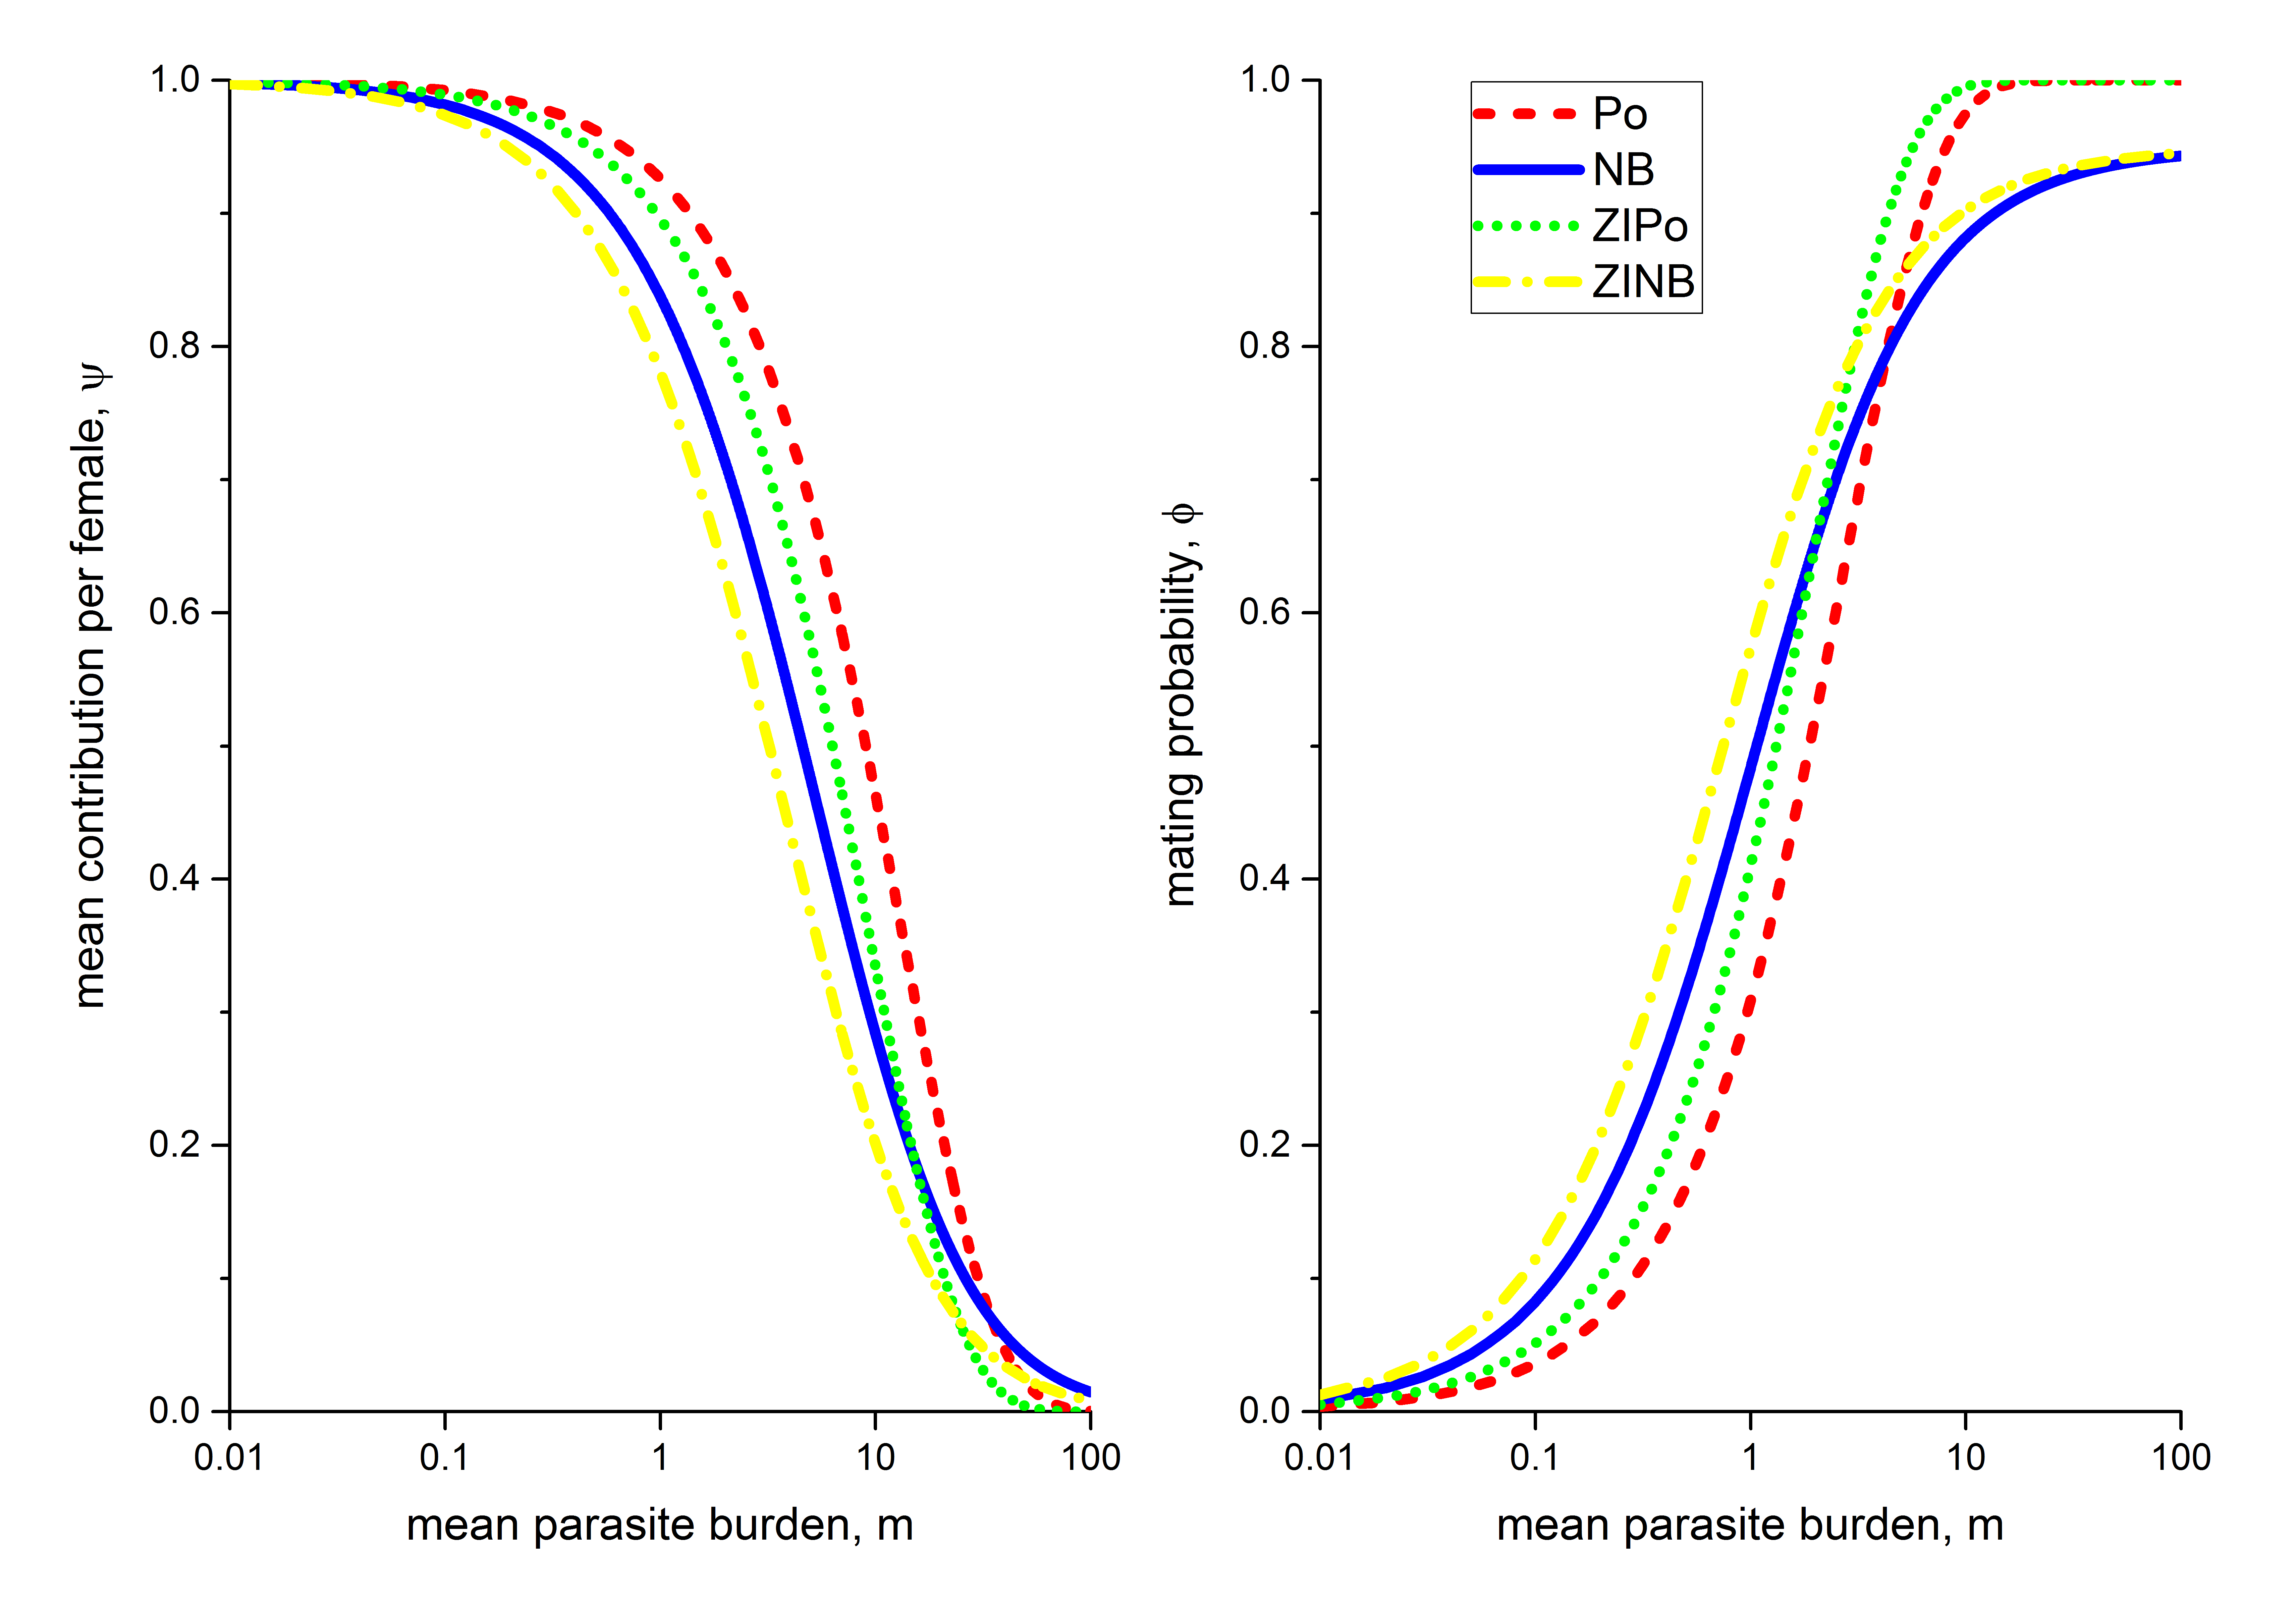
\includegraphics[width=0.99\linewidth]{functionv3}
		\caption{The mean effective contribution per female parasite, $\psi$ (left) and the mating probability, $\phi$ (right) corresponding to Poisson (dash curve), negative binomial (solid curve), zero-inflated Poisson (dot curve) and zero-inflated negative binomial (dash dot curve) distributions. All as a function of mean parasite burden $m$.}
		\label{fig:phi}
	\end{figure}

%	\subsection{Otras distribuciones simples}
%	Consideremos primero el caso de la distribución logarítmica, donde su fgp es de la forma 
%	\begin{equation*}
%	\begin{split}
%	G(s)&=\frac{\ln(1-ps)}{\ln(1-p)}\\
%	%G'(s)&=\frac{-1}{\ln(1-p)}\frac{p}{1-ps}
%	\end{split}
%	\end{equation*}
%	Entonces la probabilidad de apareamiento general $\phi$ y  la producción de huevos $\psi$ vienen dadas por las expresiones
%	\begin{equation*}
%	\begin{split}
%	\psi&= \frac{1-p}{1-pz} \\
%	\phi&=1-\frac{1-pz}{1-p\alpha z} 
%	\end{split}
%	\end{equation*}
%	
%	Otro ejemplo es considerar la distribución binomial, con fgp dada por
%	\begin{equation*}
%	\begin{split}
%	G(s)&=\left[1+ p(s-1)\right] ^n \\
%	%G'(s)&=np \left[  1+ p(s-1)\right]^{n-1}
%	\end{split}
%	\end{equation*}
%	Por lo tanto la probabilidad de apareamiento general $\phi$ y  la producción de huevos $\psi$ para este caso estan dadas por 
%	\begin{equation*}
%	\begin{split}
%	\psi&=\left[ 1+ p(z-1)\right]^{n-1} \\ 
%	\phi&=1-\left[\frac{1+ p(\alpha z-1)}{1+ p(z-1)} \right]^{n-1} 
%	\end{split}
%	\end{equation*}
%	A continuación en la Figura \ref{fig:phi} vamos a mostrar un gráfico de la contribución media por hembra $\psi$ y la probabilidad de apareamiento $\phi$ para todas las distribuciones que tratamos.   
%	\begin{figure}[h!]
%		\centering
%		\includegraphics[width=0.49\linewidth]{psinegativa}
%		\includegraphics[width=0.49\linewidth]{mating}
%		\caption{La contribución media por hembra a la izquierda y la probabilidad de apareamiento a la derecha, ambas como función de la carga media de parásitos}
%		\label{fig:phi}
%	\end{figure}

%%%%%%%%%%%%%%%%%%%%%%%%%%%%%%%%%%%%%%%%%%%%%%%%%%%%%%%%%%%%%%%%%%

\section{Independence in the variables $F$ and $M$}\label{sec:disindep}
Let $W$ be the random variable count of the number of parasites in a host and $F$, $M$ are the number of female and male parasites, respectively.
In section \ref{sec:distsexo} we assumed that we know the parasite distribution in host, $W=F+M$, and therefore  the variables F and M are not independent.
%In section  \ref{sec:distsexo} we assumed that the variables $F$ and $M$ were dependent. 
In this section we study the case in which these variables are independent, that is, $W$, $F$ and $M$ verify the following properties
\begin{equation}\label{independencia}
\begin{split}
W&=F+M\\
G_W(s)&=G_F(s)G_M(s)
\end{split}
\end{equation}
The independence of the variables $F$ and $M$ can occur when the parasites are acquired individually, as in case of hookworm parasites that can penetrate the skin of host \cite{bethony2006soil,hotez2004hookworm}.



We present all the expressions developed in the sections \ref{sec:distsexo} and \ref{sec:probapareamiento}, proofs  are  in the Appendix %\eqref{formulasind}
\begin{itemize}
	\item Mean number of fertilized female parasites
	\begin{align}
	%\sum_{i\geq 1}\sum_{j\geq 0} j p_F(j)p_M(i)=
	\alpha m \left[1-p_M(0) \right] 
	\end{align}
	
	\item Mating probability 
	\begin{align}
	%\frac{\sum_{i\geq 1}\sum_{j\geq 0} j p_F(j)p_M(i)}{\sum_{j\geq 0} j p_F(j)}=
	1-p_M(0) 
	\end{align}
	
	\item Mean egg production per host
	\begin{equation}
	\lambda_0G_M(z)G'_F(z)
	\end{equation}
	
	\item Mean fertilized egg production
	\begin{equation}
	\lambda_0 G_M(z) G'_F(z)\left[ 1-\frac{p_M(0)}{G_M(z)}\right]
	\end{equation}
	
	\item Mean effective transmission contribution by female parasite
	\begin{align}
	\psi=\frac{G_M(z)G'_F(z)}{\alpha m}
	\end{align}
	
	\item Mating probability and density-dependence effects
	\begin{equation}
	\phi= 1-\frac{p_M(0)}{G_M(z)}
	\end{equation}
	
	\item Contribution of mean fertilized egg production for mean-based deterministic model  of parasite burden
	\begin{equation}
	\lambda_0 \alpha m \psi(m) \phi(m)
	\end{equation}
\end{itemize}


\subsection{Some examples}
%Assuming that F and M have the same statistical model, the independence of the variables does not ensure that their sum of these variables
%corresponds to the same statistical model.

Distributions for the variables $F$ and $M$ are expected to be the same, but with different parameter values if the sex ratio it is not 1:1. However the total parasite burden distribution ($M$), obtained from the conditions \eqref{independencia}, may have a different distribution. 



In the examples presented here we show some cases where the variables $W$ , $F$ and $M$ have all the same statistical model.
We work with some of the most popular distributions	used to model parasites and in all cases and arbitrary sex ratio $\alpha:\beta$, where $\alpha+\beta=1$, it is assumed. 

%	Suponiendo que $F$ y $M$ pertenezcan a una misma familia de distribuciones, la independencia de estas variables aleatorias no asegura que la suma pertenezca a esta familia. En los ejemplos que presentaremos aquí se pretende que las variables $W$, $F$ y $M$ pertenezcan a una misma familia de distribuciones.
%	A modo de ejemplo trabajaremos con algunas de las distribuciones más utilizadas. Recordemos que suponemos que las proporciones sexuales de los parásitos \textit{hembra : macho} son $\alpha:\beta$, donde $\alpha+\beta=1$.  
\subsubsection{Poisson}
For the case where the distribution of parasites per host is Poisson with mean $\lambda$, that is, $W\sim \mathrm{Po}(\lambda)$. A solution for the independence of variables $F$ and $M$ are the following distributions
%Para el caso donde la distribución de parásitos en una comunidad de hospedadores sea Poisson con media $\lambda$, es decir, $W\sim \mathrm{Po}(\lambda)$. Una solución de para la independencia de las variables $F$ y $M$ son las siguiente distribuciones       
%	\begin{equation*}
%	F\sim \mathrm{Po}(\alpha \lambda) \qquad M\sim \mathrm{Po}(\beta \lambda)
%	\end{equation*}
%	\begin{align*}
%	G_F(s)G_M(s)&=e^{\alpha\lambda(s-1)}e^{\beta\lambda(s-1)}\\
%	&=e^{(\alpha+\beta)\lambda(s-1)}\\
%	&=e^{\lambda(s-1)}\\
%	&=G_W(s)
%	\end{align*}
\begin{equation*}
F\sim \mathrm{Po}(\alpha \lambda) \qquad M\sim \mathrm{Po}(\beta \lambda)
\end{equation*}
\begin{align*}
G_F(s)G_M(s)&=e^{\alpha\lambda(s-1)}e^{\beta\lambda(s-1)}\\
&=e^{(\alpha+\beta)\lambda(s-1)}\\
&=e^{\lambda(s-1)}\\
&=G_{F+M}(s)\\
&=G_W(s)
\end{align*}
Note that the pgf of $F$ and $M$ coincide with what was obtained in section \ref{sec:distsexo}, which shows the independence of these variables in that section.
We show some of the expressions obtained in the previous section \ref{sec:distsexo} for this case:
%associated with the distributions by sex	
%Notemos que las fgp de $F$ y $M$ coincide con la obtenida en la sección \ref{sec:distsexo}, lo cual muestra la independencia de estas variables en esa sección. 
%Mostramos algunas de las expresiones obtenidas en la sección anterior para el caso de independencia entre las variables asociadas a las distribuciones por sexo %de la carga parasitaria por hospedador 
\begin{itemize}
	\item Mean effective transmission contribution by female parasite
	\begin{align*}
	\psi=\frac{G_M(z)G'_F(z)}{G'_F(1)}=e^{-m(1-z)}
	\end{align*}
	
	\item Mating probability and density-dependence effects
	\begin{equation*}
	\phi= 1-\frac{p_M(0)}{G_M(z)}=1-e^{- m  z \beta}
	\end{equation*}
\end{itemize}
Note that the expression for $\psi$ and $\phi$ are the same as those obtained in the section \ref{sec:ejemplos}.
%Notemos que la expresión de $\psi$ y $\phi$ son los mismo obtenidos en la sección \ref{sec:ejemplos}.

\subsubsection{Negative binomial}

If $F$ and $M$ are negative binomial distributed with parameters $m_F=\alpha m$, $k_F=\alpha k$, $m_M=\beta m$, $k_M=\beta k$, 
\begin{equation*}
F\sim \mathrm{NB}(\alpha m,\alpha k) \qquad M\sim \mathrm{NB}(\beta m,\beta k)
\end{equation*}  
Then the distribution of $W=F+M$ is the negative binomial distribution with parameters $m$ and $k$. In fact,  a solution to problem (\ref{independencia}) is given by

\begin{align*}
G_F(s)G_M(s)&=\left[ 1-\frac{\alpha m}{\alpha k}(s-1)\right] ^{-\alpha k} \left[ 1-\frac{\beta m}{\beta k}(s-1)\right] ^{-\beta k}\\
&=\left[ 1-\frac{m}{k}(s-1)\right] ^{-\alpha k-\beta k}\\
&=\left[ 1- \frac{m}{k}(s-1) \right] ^{-k}\\
&=G_{F+M}(s)\\
&=G_W(s)
\end{align*}
For this case, the pgf of $F$ and $M$ are not equal to those obtained in section \ref{sec:distsexo}, since it was shown that the variables were not independent. We show some of the expressions obtained in the previous section \ref{sec:distsexo} for case of independence between variables 
\begin{itemize}
	\item Mean effective transmission contribution by female parasite
	\begin{align}
	\psi=\frac{G_M(z)G'_F(z)}{\alpha m}=\left[ 1-\frac{m}{k}(z-1)\right] ^{-(k+1)}
	\end{align}
	
	\item Mating probability and density-dependence effects
	\begin{equation}
	\phi= 1-\frac{p_M(0)}{G_M(z)}=1-\left[ \frac{1+\frac{m}{k}}{1-\frac{m}{k}(z-1)}\right]^{-\beta k} 
	\end{equation}
\end{itemize}
Note that the expression $\psi$ is the same one obtained in the section \ref{sec:ejemplos}.

In Figure \ref{fig:funphi} we show the behavior of the mating probability function for the cases in which the female and male parasites are distributed together or independently.
\begin{figure}
%\centerline{
\includegraphics[width=2.25in]{mouse.eps}}
		\centering
		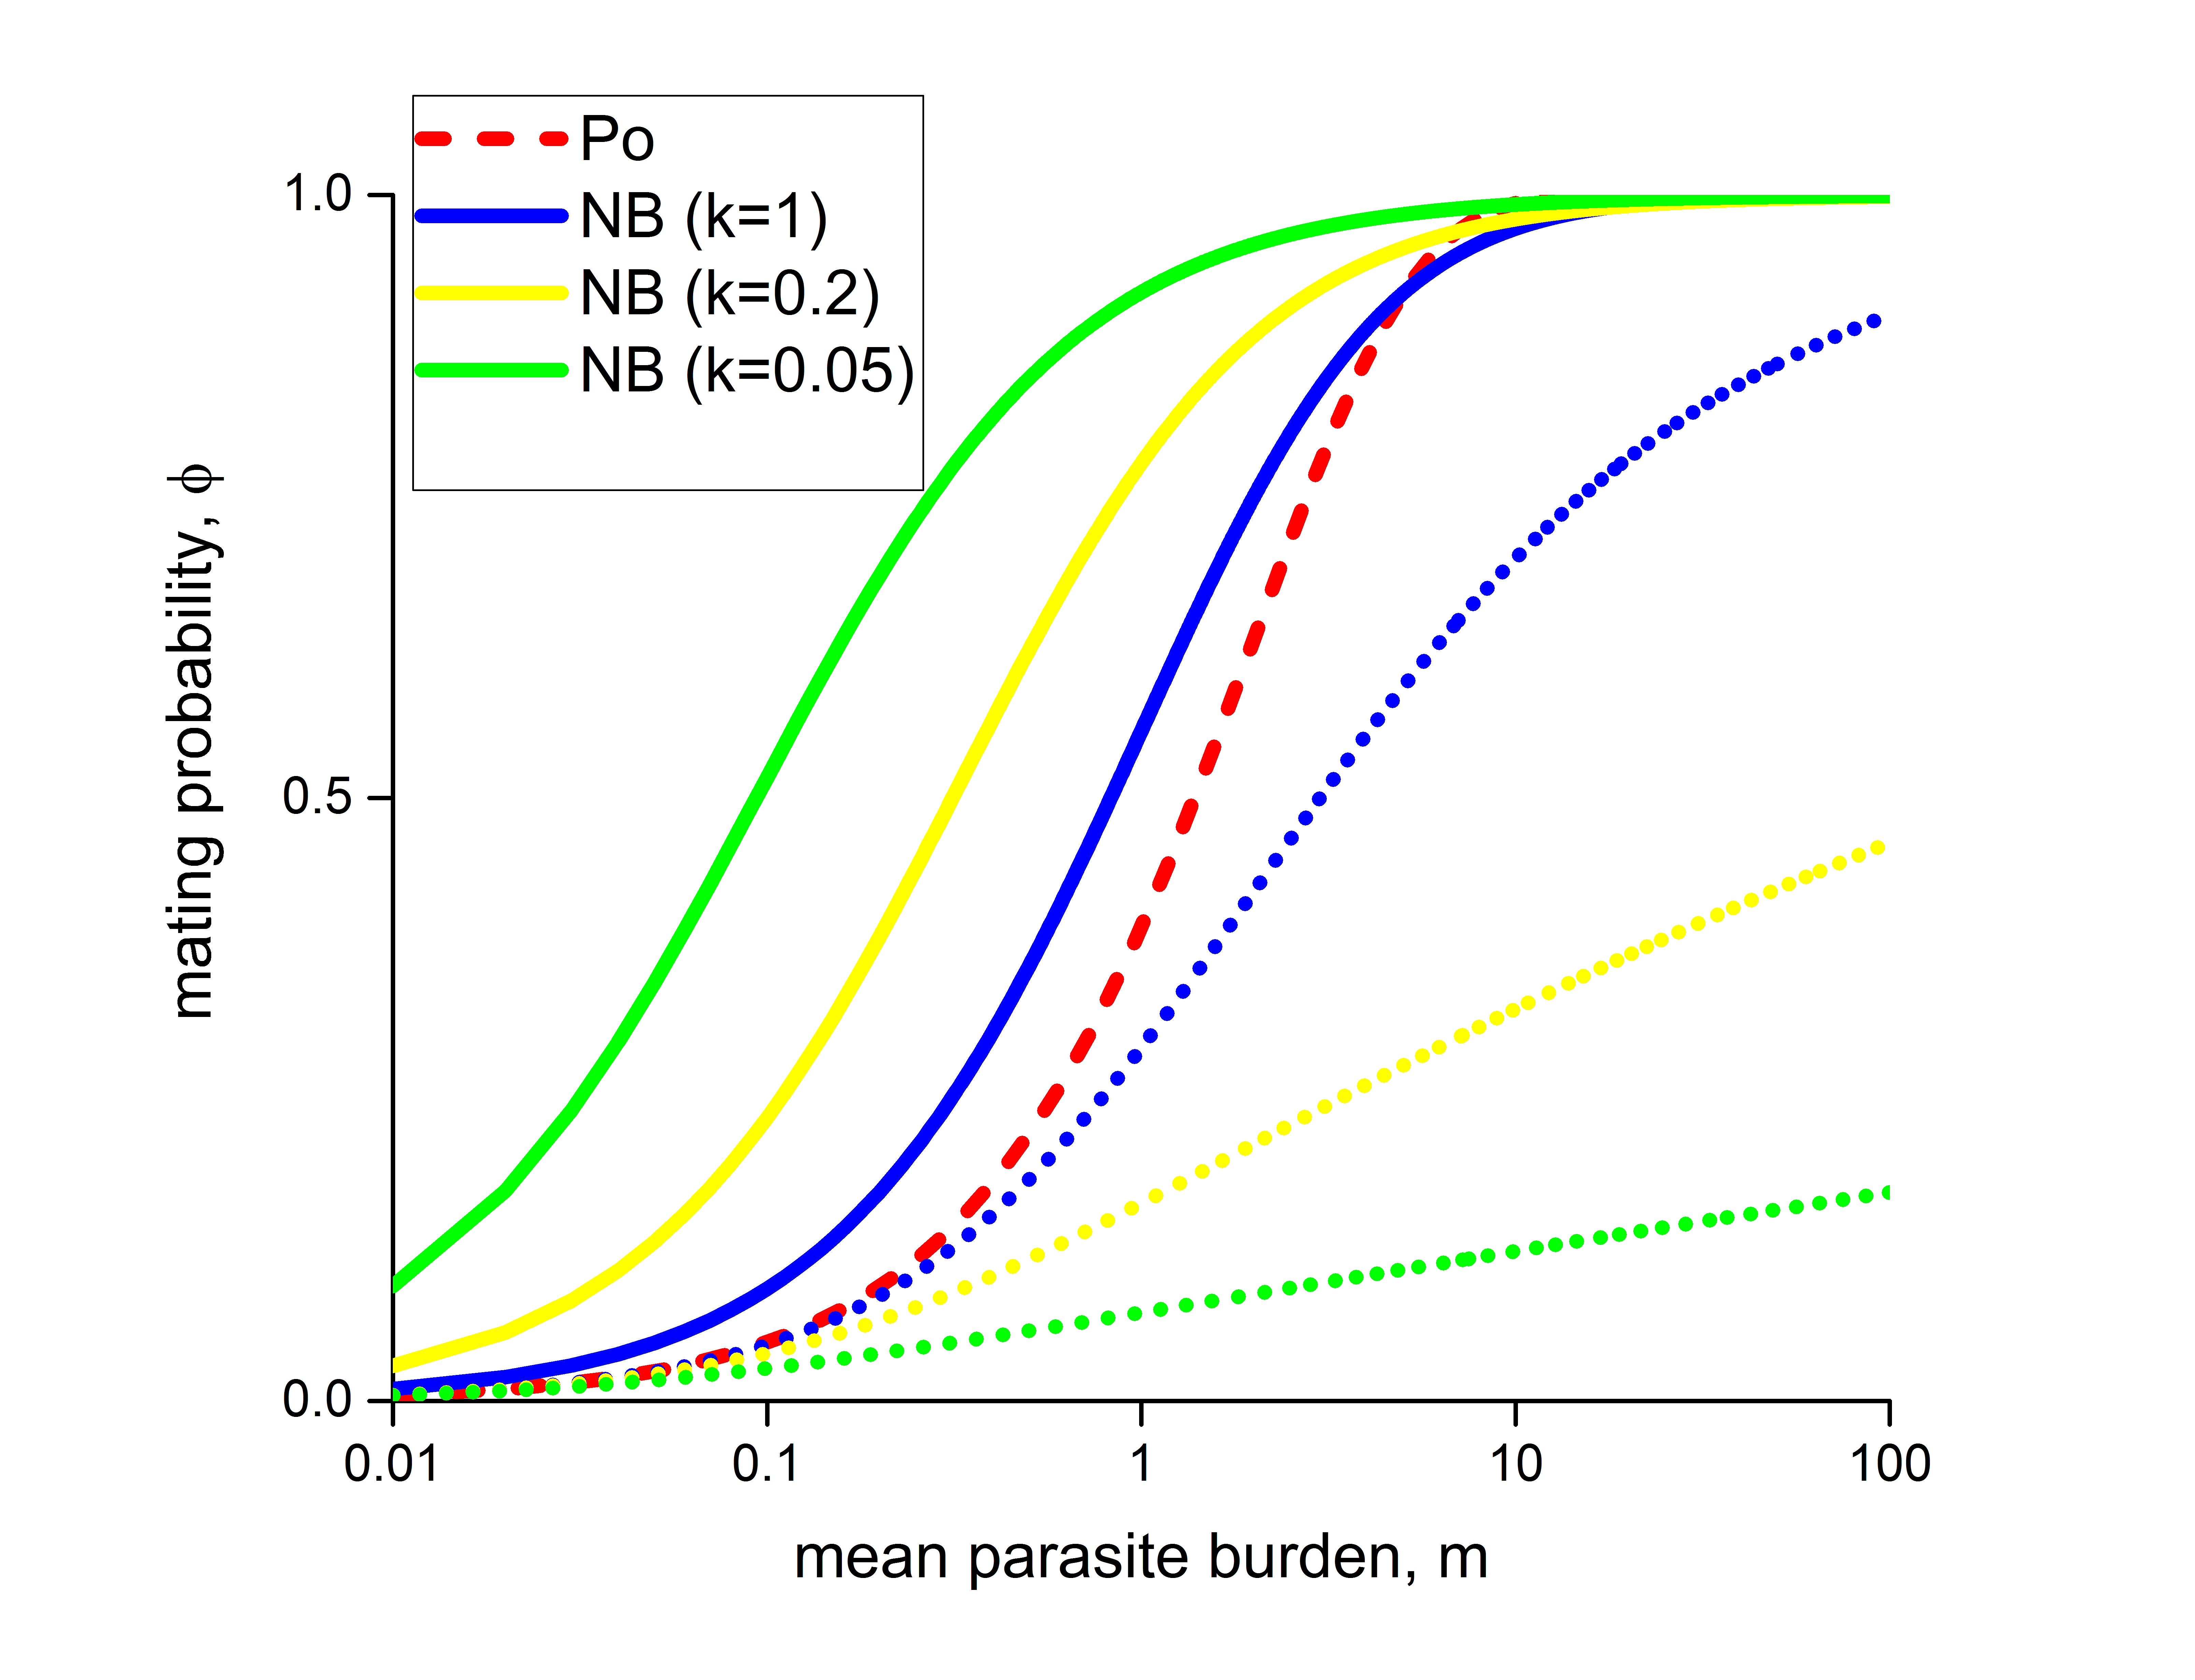
\includegraphics[width=0.99\linewidth]{phi-inde}
		\caption{Mating probability as a function of mean parasite burden $m$. The dashed curve (red) corresponds to a Poisson distribution ($k\to \infty$). 
		%{\color{red}
		The solid and dotted curves correspond to a negative binomial distribution with joint or independent distribution by sex, respectively, where $k = 1$ (blue), $k =0.2$ (yellow) and $k =0.05$ (green).
		%}
		} 
		\label{fig:funphi}
\end{figure}
\section{Discussion and Conclusions}


In most cases total macroparasites distribution is determined by the infection process and therefore the variables $F$ and $M$ (number of female and male parasites within the host) are not independent variables. We presented a general form to obtain the parasite female burden distribution in hosts from the observed total parasite distribution. 	

Different reproductive variables of parasites of importance for population dynamics, such as the mean number of fertilized female parasites, mean egg production, mating probability, mean fertilized egg production and mating probability, were obtained. 

The  expressions obtained for these reproductive variables in the different examples are generalizations (for the case of density-dependent fertility on reproductive behavior of parasites) of those obtained in \cite{leyton1968stochastic,may1977togetherness,may1993biased}.


%%%%%%%%%%%%%%%%%%%%%%%%%%%%%%%%%%%%

When parasites are acquired individually we expect the random variables $F$ and $M$ to be independent. We also expect that these variables have the same type of distribution. 


But the total host parasite burden $W=F+M$ not necessarily will inherit the same distribution os $F$ and $M$. There are some obvious cases where it is known that the distribution of the sum of random variables have the same distribution of the the variables like in the case of independent Poisson distributed variables. However for the important case of negative binomial distributed variables this is not generally true. In this work we show that 
%{\color{red} only?} if 
only if
$F\sim \mathrm{NB}(\alpha m,\alpha k)$ and $ M\sim \mathrm{NB}(\beta m,\beta k)$ then the total burden is negative binomial distributed with parameters $m$ and $k$. 


%%%%%%%%%%%%%%%%%%%%%%%%%%%%%%

One of the main limitations of this work is that it only considers parasites with a polygamous mating system and we do not consider monogamous and hermaphroditic parasites.

%{\color{red}	
In conclusion, in this work we obtained a general expression for egg production and the mating probability of the parasites. We show how these expressions depend on the sex distribution of the parasites and whether these distributions are considered joint or independent. 
We also show that these expressions vary due to the effects of the density-dependence of the parasites.
%}	

\


%\section{Inference}
%\label{s:inf}
%
%Please see the file \texttt{biomsample.tex} for fancy examples of making
%tables.  Here is a very simple one.  Use \texttt{table} for tables
%that are narrow enough to fit in one column of the typeset journl; use
%\texttt{table*} for tables that need to span two columns.  For
%figures, use of \texttt{figure} and \texttt{figure*} is analogous. 
%
%\begin{table}
%\caption{This is a simple table.}
%\label{t:one}
%\begin{center}
%\begin{tabular}{lrrr}
%\Hline
%Estimator & \multicolumn{1}{c}{$\beta_1$} &  \multicolumn{1}{c}{$\beta_2$} & 
%\multicolumn{1}{c}{$\beta_3$} \\ \hline
%MLE & 10.18 & $-$3.26 & 0.13 \\
%OLS & 9.92 & $-$3.19 & 0.11 \\
%WLS & 9.88 & $-$3.33 & 0.12 \\
%\hline
%\end{tabular}
%\end{center}
%\end{table}

%You can experiment with fancier tables than Table~\ref{t:one}.
%
%We can get bold symbols using \verb+\bmath+, for example, $\bmath{\alpha}_i$.
%
%\section{Discussion}
%\label{s:discuss}
%
%Put your final comments here. 

%  The \backmatter command formats the subsequent headings so that they
%  are in the journal style.  Please keep this command in your document
%  in this position, right after the final section of the main part of 
%  the paper and right before the Acknowledgements, Supporting Information (Supplementary %  Materials),   and References sections. 

\backmatter

%  This section is optional.  Here is where you will want to cite
%  grants, people who helped with the paper, etc.  But keep it short!

\section*{Aknowledgements}

This work was partially supported by grant CIUNSA 2018-2467. JPA is a member of the CONICET. GML is a doctoral fellow of CONICET.
\vspace*{-8pt}

%\section*{Conflict of Interest}
%
%The authors have declared no conflict of interest.
%\vspace*{-8pt}

%\section*{Acknowledgements}
%The authors thank Professor A. Sen for some helpful suggestions,
%Dr C. R. Rangarajan for a critical reading of the original version of the
%paper, and an anonymous referee for very useful comments that improved
%the presentation of the paper.\vspace*{-8pt}



%  Here, we create the bibliographic entries manually, following the
%  journal style.  If you use this method or use natbib, PLEASE PAY
%  CAREFUL ATTENTION TO THE BIBLIOGRAPHIC STYLE IN A RECENT ISSUE OF
%  THE JOURNAL AND FOLLOW IT!  Failure to follow stylistic conventions
%  just lengthens the time spend copyediting your paper and hence its
%  position in the publication queue should it be accepted.

%  We greatly prefer that you incorporate the references for your
%  article into the body of the article as we have done here 
%  (you can use natbib or not as you choose) than use BiBTeX,
%  so that your article is self-contained in one file.
%  If you do use BiBTeX, please use the .bst file that comes with 
%  the distribution.  In this case, replace the thebibliography
%  environment below by 
%
 \bibliographystyle{biom} 
 \bibliography{biblio}

%\begin{thebibliography}{}
%
%\bibitem{ } Cox, D. R. (1972). Regression models and life tables (with
%discussion).  \textit{Journal of the Royal Statistical Society, Series B}
%\textbf{34,} 187--200.
%
%\bibitem{ }  Hastie, T., Tibshirani, R., and Friedman, J. (2001). \textit{The 
%Elements of Statistical Learning: Data Mining, Inference, and Prediction}.
%New York: Springer.
%
%\end{thebibliography}

%  If your paper refers to supporting web material, then you MUST
%  include this section!!  See Instructions for Authors at the journal
%  website http://www.biometrics.tibs.org


%\section*{Supporting Information}
%
%Web Appendix A, referenced in Section~\ref{s:model}, is available with
%this paper at the Biometrics website on Wiley Online
%Library.\vspace*{-8pt}

\appendix

%  To get the journal style of heading for an appendix, mimic the following.

%\section{Appendix}
\section{}
We will assume that $p$ is the probability mass function of the distribution of parasites per host and $G$ its probability generating function.
%	En lo que sigue de esta sección supondremos que la 
%	distribución de parásitos de la población de hospedadores tiene asociada a
%	$p$ como la función de masa de probabilidad (fmp), mientras que $G$ es la función generadora de probabilidad (fgp). 

\subsection{Mean number of fertilized female parasites}%\label{hembrasfecun}
%\begin{prop}
%\label{hembrasfecun}
	%Sean $p$ la fmp de la distribución de parásitos y $G$ su fgp, entonces el número medio de parásitos hembra fecundadas por hospedador esta dado por
	The mean number of fertilized female parasites is given by     
	\begin{equation}\label{hembrasfecun}
	\alpha  m - \alpha G'(\alpha)
	\end{equation}
	%\begin{proof}
		Proof: The presence of at least one male parasite in the host ensures the fertility of all females, so
		%The presence of at least one male parasite in the host ensures that all females will be fertilized, so
		%La presencia de uno o más parásitos macho en el hospedador es suficiente para asegura que todas las hembras serán fecundadas, entonces el número medio de parásitos hembra fecundadas por hospedador esta dado por
		\begin{equation*}
		\begin{split}
		\sum_{n\geq 0}\sum_{j=1}^{n-1}j p_n\binom{n}{j}\alpha^j\beta^{n-j}
		%&=\sum_{n\geq 0}\sum_{j=1}^{n-1}jp(n)\binom{n}{j}\alpha^j\beta^{n-j}\\
		&=\sum_{n\geq 0}p_n\sum_{j=1}^{n-1} j\binom{n}{j}\alpha^j\beta^{n-j}\\
		&=\sum_{n\geq 0}p_n(n\alpha-n\alpha^n)\\
		\end{split}
		\end{equation*}
		where the last line is obtained from the expression of the mean of $\mathrm{B}(n,\alpha)$, $n\alpha=\sum_{j=0}^{n} j\binom{n} {j}\alpha^j\beta^{n-j}$. Therefore
		%donde la ultima linea se obtiene de la expresión de la media de la $\mathrm{B}(n,\alpha)$,  $n\alpha=\sum_{j=0}^{n} j\binom{n}{j}\alpha^j\beta^{n-j}$. Por lo tanto 
		\begin{equation*}
		\begin{split}
		\sum_{n\geq 0}\sum_{j=1}^{n-1}jp_n\binom{n}{j}\alpha^j\beta^{n-j}
		&=\alpha\sum_{n\geq 0}np_n(1-\alpha^{n-1})\\
		&=\alpha \left[ \sum_{n\geq 0}np_n-\sum_{n\geq 0}n\alpha ^{n-1}p_n\right] \\
		&= \alpha  m - \alpha G'(\alpha) 
		\end{split}
		\end{equation*}
	%\end{proof}
%\end{prop}
\subsection{Mean egg production per host}
%\begin{prop}\label{prodhuevos}
	%Sean $p$ la fmp de la distribución de parásitos sobre una población de hospedadores y $G$ su fgp, la producción media de huevos por hospedador esta dada por
	The mean egg production per host is given by
	\begin{equation}\label{prodhuevos}
	\lambda_0\alpha G'(z)
	\end{equation}
	%\begin{proof}
		%Consideramos que todas las hembras presentes en el hospedador pueden producir huevos según su fecundidad per cápita
		Proof: We consider that all females present in the host can produce eggs according to their  per-capita fecundity
		\begin{equation*}
		\begin{split}
		\sum_{n\geq 0}\sum_{j=0}^{n}j\lambda(n)p_n\binom{n}{j}\alpha^j\beta^{n-j}
		&=\lambda_0\sum_{n\geq 0}\sum_{j=0}^{n}jz^{n-1}p_n\binom{n}{j}\alpha^j\beta^{n-j}\\
		&=\lambda_0\sum_{n\geq 0}z^{n-1}p_n\sum_{j=0}^{n} j\binom{n}{j}\alpha^j\beta^{n-j}\\
		&=\lambda_0\sum_{n\geq 0}z^{n-1}p_nn\alpha\\
		&=\lambda_0\alpha  \sum_{n\geq 0}nz^{n-1}p_n \\
		&=\lambda_0\alpha G'(z)
		\end{split}
		\end{equation*}
	%\end{proof}
%\end{prop}

\subsection{Mean fertilized egg production per host}
%\begin{prop}
	
	%Sean $p$ la fmp de la distribución de parásitos sobre una población de hospedadores y $G$ su fgp, la producción media de huevos fecundados por hospedador esta dada por
	The mean fertilized egg production per host is given by
	\begin{equation}\label{prodhuevosfecun}
	\lambda_0\alpha G'(z)\left[1-\frac{G'(\alpha z)}{G'(z)} \right]
	\end{equation}
	%\begin{proof}
		Proof: Identical to the previous demonstration but considering only fertilized females
		%Idéntica a la demostración anterior pero considerando solo hembras fecundadas
		\begin{equation*}
		\begin{split}
		\sum_{n\geq 0}\sum_{j=1}^{n-1}j\lambda(n)p_n\binom{n}{j}\alpha^j\beta^{n-j}
		&=\lambda_0\sum_{n\geq 0}\sum_{j=1}^{n-1}jz^{n-1}p_n\binom{n}{j}\alpha^j\beta^{n-j}\\
		&=\lambda_0\sum_{n\geq 0}z^{n-1}p_n\sum_{j=1}^{n-1} j\binom{n}{j}\alpha^j\beta^{n-j}\\
		&=\lambda_0\sum_{n\geq 0}z^{n-1}p_n(n\alpha-n\alpha^n)\\
		%\end{split}
		%			\end{equation*}
		%			donde la ultima linea se obtiene de la expresión de la media de $\mathrm{B}(n,\alpha)$,  $n\alpha=\sum_{j=0}^{n} j\binom{n}{j}\alpha^j\beta^{n-j}$. Por lo tanto 
		%			\begin{equation*}
		%			\begin{split}
		%			\sum_{n\geq 0}\sum_{j=1}^{n-1}j\lambda(n)p_n\binom{n}{j}\alpha^j\beta^{n-j}
		&=\lambda_0\alpha\sum_{n\geq 0}nz^{n-1}p_n(1-\alpha^{n-1})\\
		&=\lambda_0\alpha \left[ \sum_{n\geq 0}nz^{n-1}p_n-\sum_{n\geq 0}n(\alpha z)^{n-1}p_n\right] \\
		&=\lambda_0\alpha G'(z)\left[1-\frac{G'(\alpha z)}{G'(z)} \right] 
		\end{split}
		\end{equation*}
	%\end{proof}
%\end{prop}
\subsection{Independence in the variables $F$ and $M$}%\label{formulasind}
\begin{itemize}
	\item Mean number of fertilized female parasites
	\begin{align*}
	\sum_{i\geq 1}\sum_{j\geq 0} j p_F(j)p_M(i)
	&=\sum_{i\geq 1}p_M(i)\sum_{j\geq 0} j p_F(j)\\
	&=\left[1-p_M(0) \right] \alpha m
	\end{align*}
	
	\item Mating probability
	\begin{align*}
	\frac{\sum_{i\geq 1}\sum_{j\geq 0} j p_F(j)p_M(i)}{\sum_{j\geq 0} j p_F(j)}
	&=\frac{\left[1-p_M(0) \right] \alpha m }{\alpha m}\\
	&=1-p_M(0) 
	\end{align*}
	
	\item Mean egg production per host
	\begin{align*}
	\sum_{i\geq 0}\sum_{j\geq 1} j \lambda(i+j) p_F(j)p_M(i)
	&=\sum_{i\geq 0}\sum_{j\geq 1} j \lambda_0 z^{i+j-1} p_F(j)p_M(i)\\
	&=\lambda_0\sum_{i\geq 0} z^i p_M(i)\sum_{j\geq 1} j z^{j-1} p_F(j)\\
	&=\lambda_0G_M(z)G'_F(z)
	\end{align*}
	
	\item Mean fertilized egg production per host
	\begin{align*}
	\sum_{i\geq 1}\sum_{j\geq 1} j \lambda(i+j) p_F(j)p_M(i)
	&=\sum_{i\geq 1}\sum_{j\geq 1} j \lambda_0 z^{i+j-1} p_F(j)p_M(i)\\
	&=\lambda_0\sum_{i\geq 1} z^i p_M(i)\sum_{j\geq 1} j z^{j-1} p_F(j)\\
	&=\lambda_0 \left[ G_M(z)-p_M(0)\right]  G'_F(z)\\
	&=\lambda_0 G_M(z) G'_F(z)\left[ 1-\frac{p_M(0)}{G_M(z)}\right]
	\end{align*}
	
	\item Mean effective transmission contribution by female parasite
	\begin{align*}
	\psi=\frac{\sum_{i\geq 0}\sum_{j\geq 1} j \lambda(i+j) p_F(j)p_M(i)}{\sum_{j\geq 1} j p_F(j)}
	&=\frac{G_M(z)G'_F(z)}{\alpha m}
	\end{align*}
	
	\item Mating probability and density-dependence effects
	\begin{equation*}
	\phi= 1-\frac{p_M(0)}{G_M(z)}
	\end{equation*}
\end{itemize}


\label{lastpage}

\end{document}
